\part{The Robot Coworker} % Main chapter title

\label{part:robot_coworker} % Change X to a consecutive number; for referencing this chapter elsewhere, use \ref{ChapterX}

\lhead{Part 1. \emph{The Robot Coworker}} % Change X to a consecutive number; this is for the header on each page - perhaps a


In any application that is not entirely composed by repetitive, precomputed actions, robots need reasoning skills, which severely depend on the quality of the representation of the current environment. This representation can be more or less complex, depending on the application. 

Imagine, for example, a robot whose task is cleaning the floor of a room. In the simplest case, this robot would only be provided with an elementary set of sensors. Without the capacity to understand which areas actually need cleaning, this robot could only move through the room, randomly or with some strategy, achieving the task in a longer amount of time than what would actually be needed. 

% In a fairly simple case, this robot would rely on a map of the room and a set of lasers, or bumper sensors, to detect obstacles. 

Now, imagine a household robot that needs to actively help a family that lives in an apartment, by fetching objects, providing information, and helping to accomplish various tasks. Let us imagine that one of the members of the family, Greg, is moving in the living room, searching around, while exclaming `Where are my glasses?'. In the ideal situation, our robot would try to help Greg, by giving him information such as `They are on the table to your right', or even by fetching them for him. 

Clearly, in this scenario, the robot needs deeper reasoning skills. It needs to understand that the user is looking for its glasses, to link them to their actual physical location, to compute the spatial relationship between the table and the glasses, and to provide information in a natural way. In fact, if the robot would tell Greg that the glasses are in the position $(3.2, 5.0 , 1.3)$, Greg would very likely be very perplexed. A more natural way would be to inform Greg that his glasses are on a table, whose location is pointed taking into account Greg's position.

In this case, having sophisticated sensors is, of course, important but not sufficient. The robot needs also to \textit{reason} on the sensor's data in order to produce meaningful information. For example: laser points and camera images need to be integrated to recognize objects and humans; spatial relationships  (e.g. the glasses are on the table) have to be properly modeled; actions performed by humans, and their effects on the environment, need to be recognized; and so on. 

The process of reasoning on data to produce symbolic information is called \textit{situation assessment}. Endsley explained in \cite{endsley1995toward} that this process is deeply linked to the quality of  decions of the robot.

While in many applications robots can benefit from a situation assessment component, being able to perform complex reasoning on data is particularly important in HRI. If the robot is able to take better decisions (i.e.  efficient, safe, socially acceptable, natural) than it will be perceived in a more positive manner by humans. 




% Chapter Template

\chapter{Plan Production and Management} % Main chapter title

\label{chapter:plan_management} % Change X to a consecutive number; for referencing this chapter elsewhere, use \ref{ChapterX}

\lhead{Chapter 4. \emph{Plan Production and Management}} % Change X to a consecutive number; this is for the header on each page - perhaps a shortened title

In this chapter, we introduce the Plan Production and Management layer of our system. Section~\ref{sec:plan_management-intro} introduces the subject, with a review on multi-agent planning, explanation, negotiation and plan management. section~\ref{sec:plan_management-overview} shows the main aspects of this component. Our system is able to use different plan management modalities, as explained in ~\ref{sec:plan_management-modalities}. section~\ref{sec:plan_management-human_knowledge} introduce the idea of maintaing the level of knowledge of a user in a task, which will be used both in plan generation and management. section~\ref{sec:plan_management-plan_generation} introduces our task planners, HATP (\ref{subsec:plan_management-hatp}), and HAPP (\ref{subsec:plan_management-happ}), and shows how plans are adapted to the expertise of humans in the  tasks (\ref{subsec:plan_generation-adapting_knowledge}). section~\ref{sec:plan_management-plan_explanation} shows how plans are explained to users, and section ~\ref{sec:plan_management-negotiation} how they are negotiated.  section~\ref{sec:plan_management-plan_manager} introduces the plan management aspects of this layer. We developed different strategies, shown in subsections ~\ref{subsec:plan_management-sequential_plan_management} and ~\ref{subsec:plan_management-adaptive_parallel_plan_manager}. section~\ref{section:plan_management-plan_monitoring} shows how are system is able to monitor human actions and task. Finally section~\ref{sec:plan_management-experiments} details a user study created to evaluate the ability of our system to adapt to users.


\section{Introduction}
\label{sec:plan_management-intro}
\subsection{Cooperation between agents}
Robots can be used to perform a large number of different operations. Some of these will be simple enough that the robot can just achieve its task by performing a prefixed sequence of elementary actions. In other cases, the robot might have to achieve complex goals, which require the ability to create plans and to adapt them to the current state of the world. When cooperating with other agents, the robot has to build a shared plan, which includes the actions that every agent need to perform, in order to coordinate and ensure the corrent achievement of the goal. We can imagine the following process:
\begin{itemize}
	\item The system receives a new goal. This can be directly introduced by a human, or chosen after some kind of reasoning by the robot.
	\item One of the agents (the robot or the humans) proposes a shared plan to achieve the goal, and presents it to the other agents.
	\item The agents negotiate the plan. In some situations, one of the agents might not be able (or might not want) to perform a specific action, or sequence of actions. The agent can refuse the plan, proposing a correction or a completely different plan.
	\item The agents execute the plan. Each agent performs its part of the plan. In addition, agents may check the state of others to monitor the correct execution of their part of the plan or to cordinate with them.
	\item An agent might fail his part of the plan. If this happens the agents need to create a new plan to account for this failure.
 	\item The process continues until the goal is achieved or it becomes unachievable (for example, a needed resource is no longer available).
\end{itemize} 
When humans cooperate this process can be very quick. For simple tasks humans are able to coordinate without explicitly forming a plan, in particular if they are used to cooperating together. Other times, when there are unexpected problems during the execution of a plan, humans are able to quickly readapt their plan, without completely restarting this process. In order to cooperate in a natural way with humans, robots need to reproduce these mechanisms.

\subsection{Multi Agent Planning}
Multi-Agent planning   is an important and studied topic in the AI community \cite{durfee1999survey}. There are several approaches to this problem, using classical or probabilistc planning. There are several issues to consider:
\begin{itemize}
\item Distributed vs Centralized. A multi-agent planner might be distributed, meaning that separate systems plan independently and then communicate to build a shared plan (an idea investigated, for example in \cite{nikolaidis2013cross,guestrin2002distributed} ); or centralized, meaning that a single system plans for all the agents.
\item Coordination. Agents need to coordinate their plans, in particular in the presence of shared resources. Imagine, for example, two agents, Max and Bob, that are using a tool to repair a set of cars. If Max is proceeding faster than Bob and the two do not coordinate, Max might take the tool and leave, starting to repair another car, ignoring the fact that Bob still needs the tool. This example shows that it is important to reason on the duration of actions performed by agents. At the simplest level, agents need to know the advancament of the sub-plan of other agents. More complex reasoning might take into account how long an agent needs to perform a certain sub-task, in order to refine a plan. 
\item Cooperation. Even when performing different sub-tasks of the same plan, agents can help each other, for example by passing items, thus improving the efficiency of the plan. Multi-Agent problems can be loosely or tightly coupled, depending on the quantity of interactions between agents. Some works are not focused specificly on tightly or loosely problems, and try to present a generic approach. \cite{torreno2015approach} proposes a cooperative refinement planning approach, based on the partial-order planning paradigm. In this work each agent refines a centralized plan. Agents are able to exchange information, since the complete world-state might no be observable by all of the agents. Refined plans are then analyzed by each agents, and voted with a democratic leadership approach. Results show that this approach is very efficient at solving loosely coupled problems, but also competent on tightly coupled situations. 

\item Communication and Knowledge. In a multi-agent environment each agent might have an incomplete or incorrent belief on the world, which might lead to wrong or sub-optimal actions. Agents may communicate to progressively build a correct belief model on the state world. 
\end{itemize}

Several approaches has been studied to bring the multi-agent planning problem in a probabilistic framework. \cite{boutilier1999sequential} create a centralized MDP, able to select at each time step actions for every present agent. Dec-POMDP \cite{bernstein2002complexity} and I-POMDP \cite{gmytrasiewicz2005framework} are more complex frameworks, that take into account the belief models of agents. The complexity of these models makes them difficult to use in even moderately difficult scenarios. A solution to this problem is considering simpler problems, where the agents mostly work independently and interact only in limited situations, such as in \cite{melo2013heuristic}.  Since we are more interested in tightly coupled scenarios, where the robot and human interact often, these kind of approaches are not suitable.

\subsection{Plan Explanation and Negotiation}
In order to form  shared plans, agents often communicate, explaining tasks to each other and negotiating to agree on a solution. In \cite{Lallee2013} the authors suggest that joint plans should be fully communicated in order to sustain effective collaboration. 

In a collaborative scenario, all the agents must agree on the shared plan. If there is a disagreement the agents might negotiate to find a nother solution.  This problem has been studied, for example, in \cite{fabregues2014hana}, where the authors present the \HANA system, an architecture that allows agents (robots and humans) to negotiate in competitive and cooperative settings. In HANA agents interact during the whole planning process, proposing solutions while they keep searching for better plans. During this process agents agree on performing specific tasks, which prunes the search space of feasible plan.

\subsection{Plan Management}
Finally, the shared plan needs to be executed. Agents need to perform their part of the plans and to monitor their partners in order to coordinate with them. Two examples of systems able to execute shared plans are  Chaski \cite{shah2011improved} and Pike \cite{levine2014concurrent,karpas2015robust}. 

Chaski is an executive system that enables the robot to anticipate and adapt to other agents actions. Chaski is based on human teamwork strategies, including ideas such least moment commitment, frequent communications on the task status, and considering the consequences of the robot's choices on other agents. Chaski is able to execute plans in two different modalities: Equal Partners and Leader and Assistant. Chaski receives as input a shared plan, including the activities that need to be performed, the capacities of each agents, and the deadlines for these activities. Chaski produced a compact representation of all the possible scheduling of activities, based on this plan, which is used to take decisions on the fly during executing, and to adapt to human choices. Results show that Chaski is able to reduce human's idle time in an equal partners scenario. A possible problem of this approach is that if an agent completely deviates from the chosen plan, the system needs to create a new plan, which needs to be encoded again by the Chaski.

Pike is another executive, able to simultaneously recognize human plans and adapt to them. Pike receives as input a plan, represented as a Temporal Plan Network with Uncertainty (TPNU). Pike represents this plans by considering controllable choices (i.e. actions) for the robot and uncontrollable choices for the human. The idea is considering that these choices are not independent, and in this way the system can infer what actions the human would rationally take to obtain his goal and what actions the robot should take to help him. The system receives a stream of human choices, which allows it to determine the robot's actions. Pike has been tested in simulation and with a real robot with good results, managing, on average, to take decisions with a low latency.

If the human does not follow the TPNU Pike will return a failure. The authors discuss integrating the system with a generative planner in the future to overcome this limitation.

\section{Overview}
\label{sec:plan_management-overview}
Our system presents a planning layer which is able to perform the following tasks:
\begin{itemize}
	\item Interface with external planners in order to create a shared plan. The system has been integrated with a HTN (Hierarchical Task Network) based planner, HATP (Human-Aware Task Planner), and with a multi-agent MDP planner.
	\item Monitor a human plan. Our system is able to monitor other agents' parts of a plan, to cordinate with them and to react when an agent fails an action or his actions diverge from the current plan.
	\item Receive plans from a user. Users can interact with the robot with a tablet application, asking it to execute specific actions or goals.
	\item Executing shared plans in different modalities. The robot can be a leader, assistant, or equal partner of humans during plan management.
\end{itemize}

A number of modules implement this ideas, as shown in figure \ref{fig:plan_management-architecture}:
\begin{itemize}
\item Task Planner. Creates a shared plan for the involved agents.
\item Plan Management. Manages the current plan, interacting with the Execution Management layer to execute the robot's action and with the Situation Assessment layer to monitor human's actions.
\end{itemize}

After receiving a goal from the Goal Management layer, the Plan Management module sends a request to the Task Planner to look for a suitable plan. If there is a plan, depending from the current modality, it will send it to the Plan Management module.. 

\begin{figure}[ht!]
	\centering
	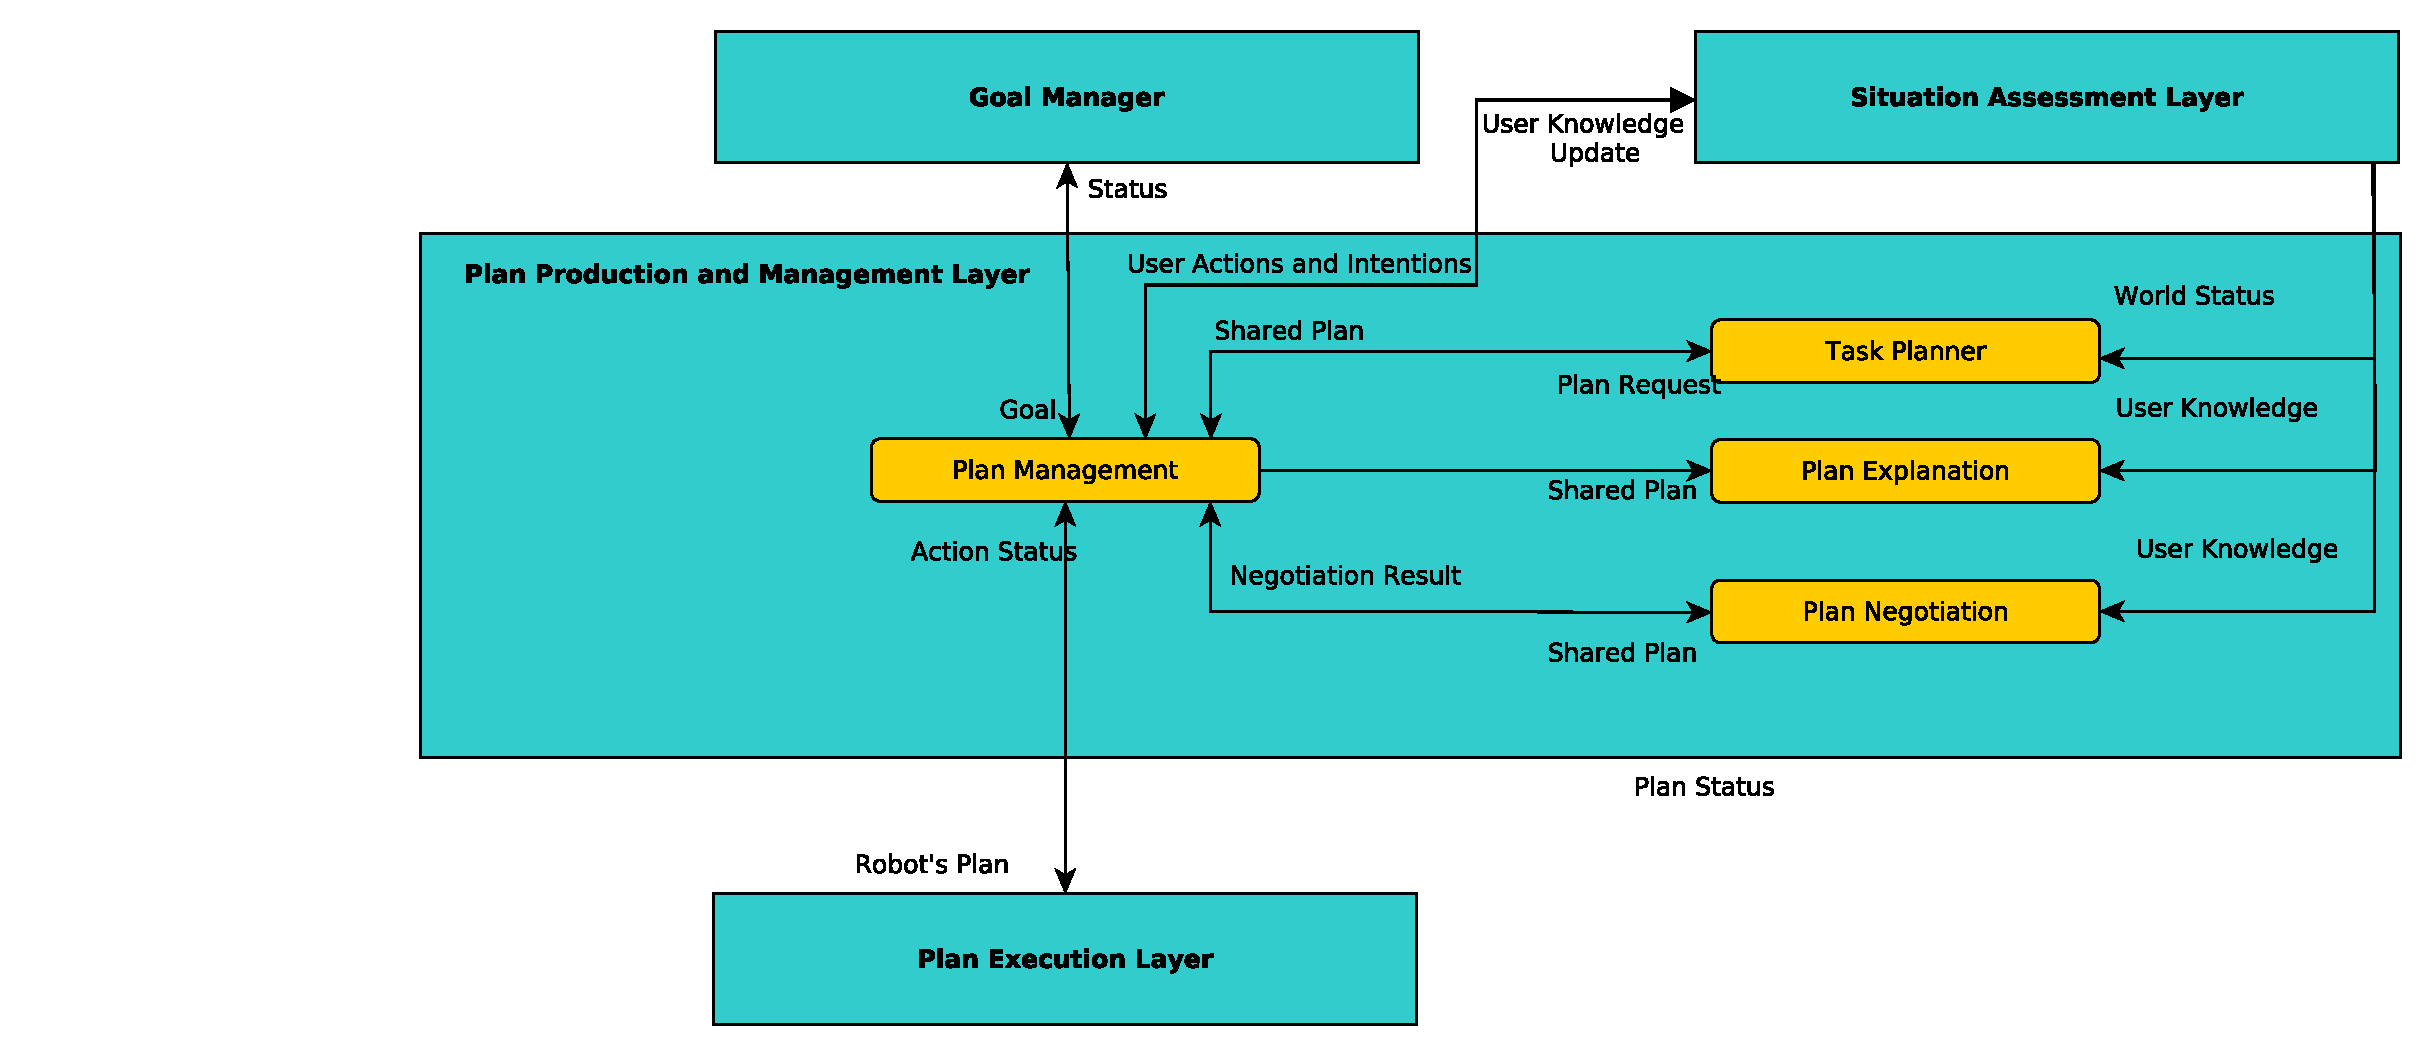
\includegraphics[scale=0.5]{img/plan_management/architecture.pdf}
	\caption[The architecture of the Plan Production and Management layer]{The architecture of the Plan Production and Management layer. Light green rounded rectangles represent modules, while dark green rectangles layers. Arrows represent message exchanged between components, with the label detailing the message.}
	\label{fig:plan_management-architecture}
\end{figure}


Part of this chapter was presented in \cite{Lallement2014,milliez2016using,fioreiser2014}.

\section{Plan Management Modalities}
\label{sec:plan_management-modalities}
When acting together, agents sometimes do not have the same decision power, with one of them assuming the role of a leader. We represent this idea, in our system, by proposing three different modalities: \textit{robot leader}, \textit{human leader}, and \textit{equal qartners}. The robot is able to switch from one modality to another during the execution of a plan. For example, if the current modality is \textit{robot leader} and the Robot receives a command from a user, it will switch to the \textit{human leader} modality, after interrupting its current action.

\subsection{Robot leader}
In this modality the robot, after computing the plan, will explain it, negotiate it and start executing it.
The robot will track the status of humans, informing them of which actions they should execute. This modality can be helpful when interacting with  naive users or in tasks where the robot has a better knowledge of the
domain or of the environment than the other agents.

\subsection{Human Leader}
The human can also create plans, interacting with the robot by using a
tablet application, as explained in section \ref{sec:situation_assessment-communication}. In this modality the robot   
will simply observe the surroundings and wait for user inputs. This modality is always available and has a priority over
the other two modalities. If the robot receives a command from the
application while it is in another modality, it will abandon its current
plan, stopping its actions at a safe point, and then execute the users'
command. We feel that this interaction modality is important for two
different reasons.  First, some users will simply prefer to be in
charge of the execution process, for a matter of personal preference or because they
feel they have a deeper knowledge on how to realize the current task
than the robot. We can picture, for example, industrial or medical
scenarios, where the human is the leader and asks the robot to perform
different tasks to help him, when needed. A second use of this modality is in situations where
the robot does not have  a clear estimation of the users' intentions and
goals. For example, in a domestic environment, a user could decide to
order a robot to bring him a drink, a need that the robot can not always anticipate.

\subsection{Equal Partners}
In the last presented operation modality the robot will try to help
the human to complete a task. At the start of the scenario, the robot
will stand still and observe the environment. After the user takes an
action the robot will calculate a plan and try to help as it can, by
performing actions related to that task and by giving helpful information to
the user, for example to fill gaps in their knowledge. In this modality, 
the robot will not explain or negotiate the current plan and will not warn humans if
their actions differ from the plan computed by the robot.

We feel that, particularly in non-critical tasks, where defining an accurate plan between the partners is not
fundamental, this modality is a very natural way of
interaction between different partners.


\section{Plan Generation}
\label{sec:plan_management-plan_generation}
One of the goals of our system is flexibility; we consider important the possibility to interface with external components. We built an intermediate Plan Generation module that interacts with external planners,  returning  plans represented in a common format that can be handled by the other modules. 

We consider that plans can be decomposed in a set of sub-parts, that we call \textit{tasks}. In general tasks can be decomposed in simpler sub-tasks, until reaching the most basic form of task of a domain, which we call \textit{action}. Both actions and tasks follow the same representations, $(name,preconditions,target,postconditions)$, that we introduced in ~\ref{chap:situation_assessment}. In ~\ref{sec:sec:situation_assessment-intention_recognition} we introduce our intention and action recognition module. In this module, we specified that the system possesses a list of known actions. Every action in a planning domain that can be performed by humans need to be present in the list posseded by the Situation Assessment module. In this way, the system will be able to monitor the execution of actions by humans, with the mechanism of the robot observer.

In some situations, to be more generic, we will use the word \textit{task} to refer to both tasks and actions, since actions are actually tasks that can not be decomposed in the current planning model.

We require that each planner, to interface with our system, provides as input a set of streams, one for each agent. A stream is a sequence of nodes, where each node corresponds to task assigned to be executed by the agent. We introduce causal links between tasks, even of different streams, to ensure synchronization. A causal link $l=(t_1,t_2)$ indicates that  $t_1$ should be execute before action $t_2$. This ensures that all the preconditions to execute $t_2$ are fullfilled. Moreover, if $t_1$ and $t_2$ are executed by different agents, and if there is a shared resource connected to the action, the causal link indicates that the resource will be released by the agent only after $t_1$ is completed. An example of these data structures is shown in figure~\ref{fig:plan_management-plan_structure}.

\begin{figure}[ht!]
 \centering
  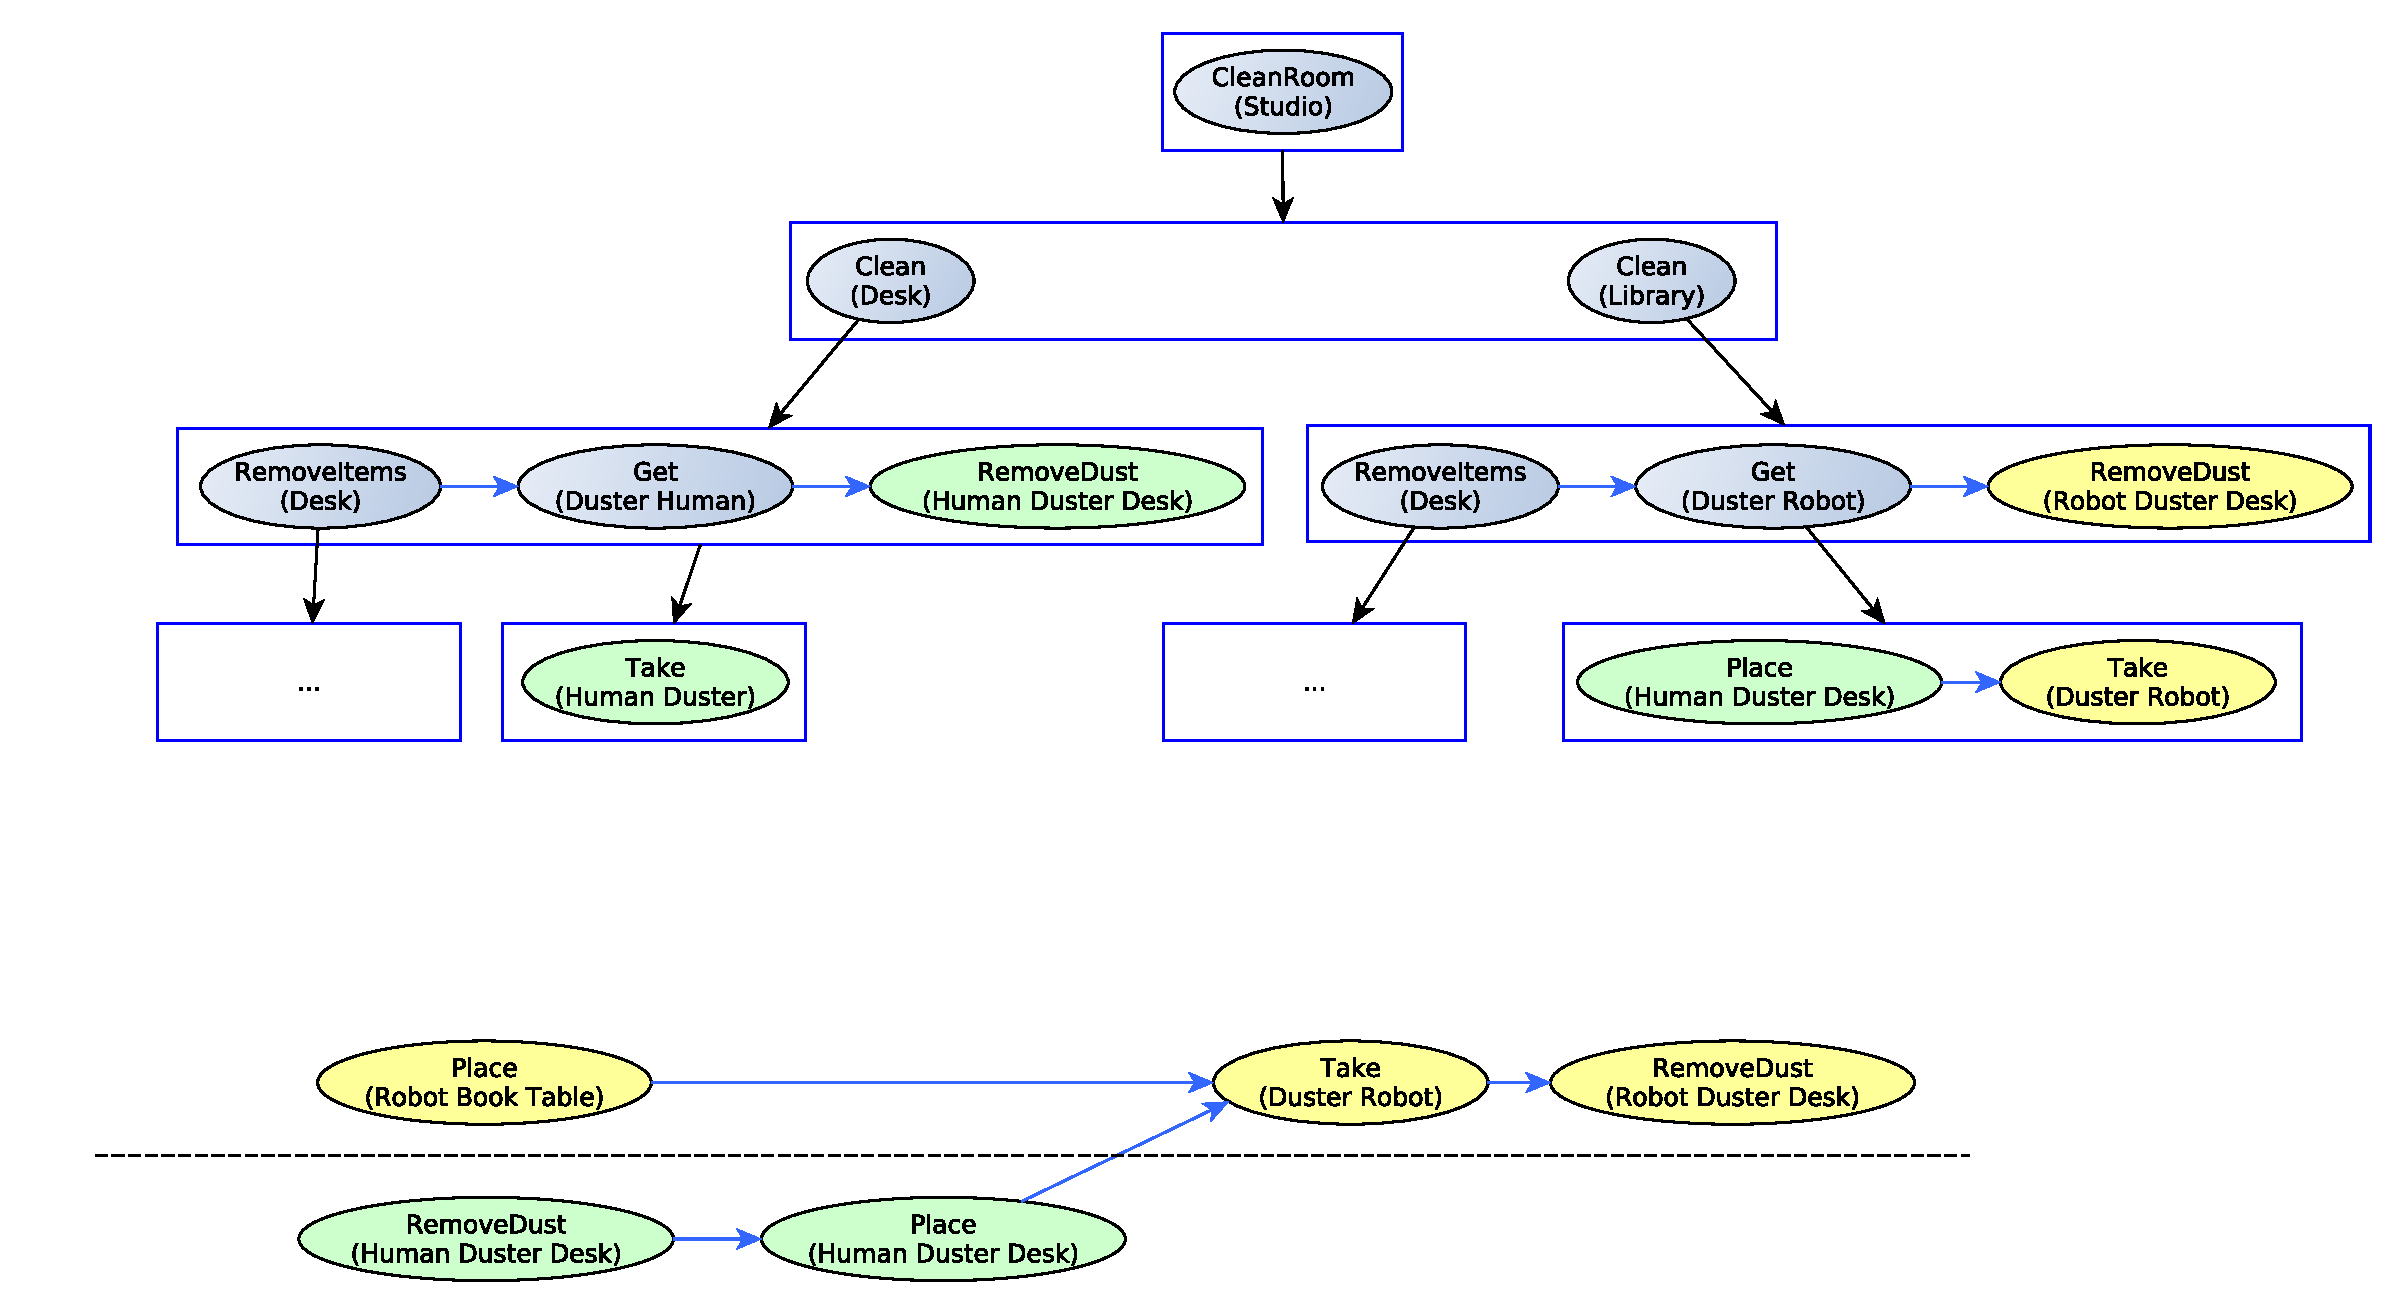
\includegraphics[scale=0.45]{img/plan_management/plan_data_example.pdf}
 \caption[Plan data structures]{a) A HTN plan data structure used in our system, representing a possible way to clean a room
 with two agents, a robot, and a human. Blue ellipses represent tasks, green ellipses represent
 actions assigned to the human, and yellow ellipses actions assigned to the robot. Each decomposition is grouped
 in a blue rectangle. Black arrows link a method to its decomposition, while blue arrows represent causal links. The two squares with a "..." label represent decompositions that are not shown in this picture.
 b) A part of the plan streams associated to the tree data structure. The upper stream represents the robot, and the lower one a human. Notice the causal link between the Place(Human Duster Desk) in the human stream and the Take(Robot Duster) in the robot stream. This link indicates that the robot should wait that the human places the duster before executing the action to take it, ensuring synchronization }
 \label{fig:plan_management-plan_structure}
 \end{figure}


At the moment, we tested two different planners with our system, which will be shown in the next subsections.


\subsection{Human-Aware Task Planner}
\label{subsec:plan_management-hatp}
Computing a plan in complex environments can be very hard and time consuming. A useful approach to reduce the search space in planning is introducing the knowledge of an expert in the system, in order to guide the planner toward desirable states. An implementation of this idea is HTN, where the domain expert specifies a hierarchical library of operations, called methods, when the operation is a node in the hierarchy, and actions, when the operation is a leaf. HATP \cite{Lallement2014} is a planning framework that extends HTN for human-robot interaction problems. Among the capacities of HATP we can find:
\begin{itemize}
\item Multi-Agent. HATP is able to include different agents in its domain, specifying which actions each one can execute. HATP is able to plan for different agents at the same time, humans and robots. The planner can also compute ``joint actions", that involves more agents at the same time.
\item Social Rules. The domain expert can introduce a set of rules, which represent desirable behaviors, for example to distribute in different ways operations between agents, or to avoid specific sequences of actions. Social rules help producing human-aware plans, that avoid behaviors that can be considered rude as humans. Using social rules, HATP can also balance in different ways the amount of effort of each agent in the plan. For example, we might choose that the human should have a minimum effort in the plan, or that the effort should be balanced between the human and the robot.
\item Cost Driven. The domain expert can specify a cost for actions. Plan pruning allows to explore more efficiently the search space, discarding paths that are not promising.
\end{itemize} 

Plans are represented as an HTN tree decomposition and as a set of streams, one per agent, which shows which actions each agent needs to perform. Casual links are introduced between streams to ensure synchronization.

\section{Plan Management}
\label{sec:plan_management-plan_manager}

The Plan Management algorithm will be divided in different threads of execution, one for each agent. We will now explain this algorithm, which is shown in figure \ref{fig:plan_management-manage_plan_not_leader}.
\begin{itemize}
  \item Each thread executes the part of the plan of an agent, composed by $n$ different actions.
  \item For each action, for every causal link $(a_i,a_n$), where $a_n$ is the current action, and $a_i$ is another action, the plan manager waits until $a_i$ is completed, or there is an error. This is handled in the \textit{waitCasualLinks} procedure.
  \item When all the causal links have been satisfied, the execute\textbackslash monitor procedure is called, depending if the thread is managing the robot or another agent. The \textit{executeAction} operation interacts with the Execution Management layer to complete the action, while the MonitorAction operation with the Situation Assessment layer.
  \item If these procedures succed, the plan manager switches to the next action, otherwise it returns a failure.
  \item The process is continued until there is a failure or the plan for the current agent is completed.
\end{itemize} 

\begin{figure}[ht!]
 \centering
 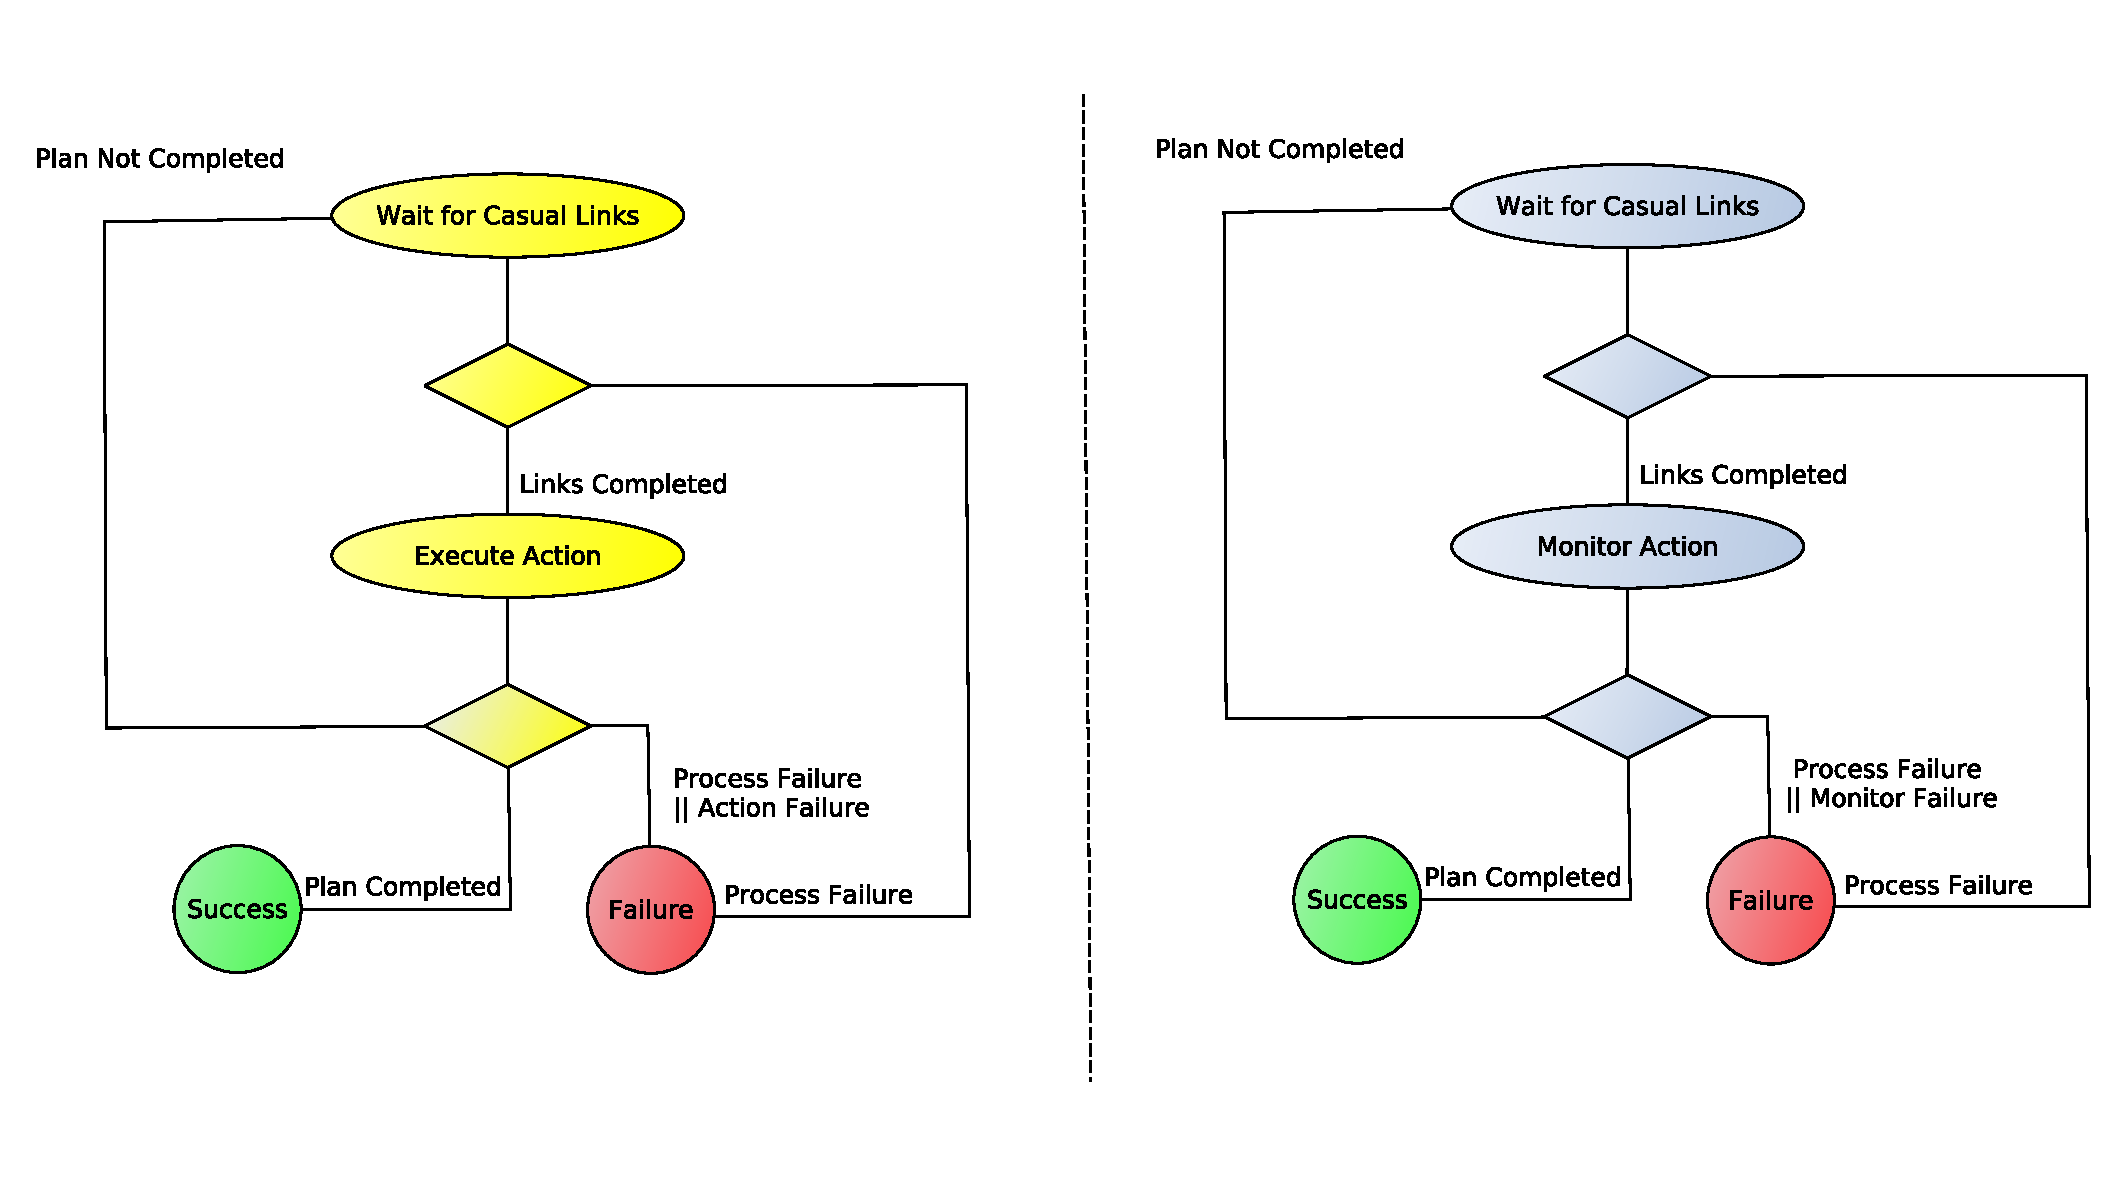
\includegraphics[scale=0.6]{img/plan_management/manage_plan_not_leader.pdf}
 \caption[Plan Management when the robot is not leader]{The plan management algorithm used when the current modality is not \textit{robot leader}. The algorithm is composed by different threads, one for each agent. In this instance, the upper lane represents the robot's management thread, while the bottom a human's management thread. Elliptic nodes represent operations. Diamond nodes, representing divergences in the algorithm, where adding only when they could simplify the understanding of the algorithm. Arrows imply a transition between nodes, with the label of the arrow representing the condition of the transition, when present. The absence of a label implies that a transition is always applied. The blue circle node, called ``start", represents the start of the algorithm. The green and red circle node, instead, represent the success or failure of the algorithm.}
 \label{fig:plan_management-manage_plan_not_leader}
 \end{figure}

Failures in the algorithm lead to a replan request. If a new plan is found, the algorithm starts again, otherwhise the goal is considered failed.

In this modality, the robot will expect users to execute a specific set of tasks, warning them if they do not respect this allocation. Sometimes, the robot will choose the decomposition of the tasks that should be executed by a user, but, when the partner is competent enough in a high-level task,  we may want to allow him the flexibility to execute it as he sees fit. 

\section{Task Monitoring}
\label{section:plan_management-plan_monitoring}

\subsection{Introduction}
During the execution of a plan, the robot will monitor other human partners. In general, having a shared plan, the robot knows what is the human's next expected action, and can monitor if it is accomplished. Plan monitoring poses a number of different issues:
\begin{itemize}
\item Understanding when the next expected action has been performed. In some situations the robot will monitor the execution of a specific action. In this event, it needs to understand when the action has been completed.
\item Understanding when the next expected task has been performed. In some situations, the robot wants to give a human cooperator the freedom to perform a subtask has he sees fit. This is a more complex problem than monitoring a specific action, since the robot needs to reason on the results of sequences of actions.
\item Evaluating the human engagement in the current task. The robot needs to understand if the human is trying to accomplish its current task, if he momentarily interrupted it, or if he abandoned it.
\end{itemize}

At the moment, we have implemented and integrated in our system only monitoring of actions. We will show how we include this idea, and then illustrate in the next chapter how we could extend our system to monitor tasks and evaluate the human engagement in the current task.

\subsection{Monitoring Actions}
At all time, as previously explained in ~\ref{chapter:situation_assessment}, the system constantly observes the environment, monitoring which actions are executed. As previously said, each action that can be executed by a human needs to have the same representation in the Situation Assessment and Plan Management layers. When the plan manager needs to monitor an action $a$ of a human stream, its $preconditions$ will be satisfied (since, if we are monitoring $a$, all of its causal links have been already satisfied). This means that $a$ will be in the IG for the human, which will be monitoring its execution.

The Plan Manager will wait for Situation Assessement to infer that an action has been performed. If the action is different from $a$, it will return an error, prompting a replan. Otherwise, the plan management will continue with the next action in the stream, if any.

For example, let us imagine a scenario where Greg is near a table, with a \textit{bottle} and a \textit{book} on top. Let us say that, at the moment, Greg can execute three actions: \textit{take book}, \textit{take bottle}, and \textit{move kitchen}. The current IG for Greg will include these actions, as well as observations to infer their execution. In this example, Greg is following the stream shown in figure. %bla.
Greg has just completed the action \textit{move to table}, and should now execute the action \textit{take bottle}, if he follows this plan. If the system infers that Greg executes \textit{take book} or \textit{move kitchen}, the plan manager will replan, since Greg executed a different action that the one that was expected. If Greg executes \textit{take book}, the stream will move to the next action, which is \textit{move kitchen}.

%ADD EXPLANATION TO SITUATION ASSESSMENT ON WHY WE USE PROBABILITIES IN ACTION RECOGNITION, and how we would use them

\subsection{Monitoring and Unseen Actions}
Often, in cooperative tasks, agents will operate in different locations, and so they can not observe each other actions all the time. Perhaps one of the agents is cooking in the kitchen,  while the robot is preparing the table for dinner. While we do not deal, in this work, with these issues, there are several studies on plan recognition in partially observable environments, like \cite{geib2005partial}.
 
% Chapter Template

\chapter{Task Execution} % Main chapter title

\label{chapter:plan_execution} % Change X to a consecutive number; for referencing this chapter elsewhere, use \ref{ChapterX}

\lhead{Chapter 5. \emph{Task Execution}} % Change X to a consecutive number; this is for the header on each page - perhaps a shortened title

This chapter shows the Task Execution layer of our system. Section \ref{sec:plan_execution-intro} introduces the subject. Section \ref{sec:plan_execution-overview} shows an overview of this layer, with its characteristics and components. Section \ref{sec:plan_execution-action_executor} shows the main aspects of the Action Execution module, while \ref{sec:plan_execution-collaborative_planners} shows the framework we use to execute human-robot joint actions.


\section{Introduction}
\label{sec:plan_execution-intro}
Acting in a human-crowded environment is a difficult problem. Even when acting independently, the robot needs to ensure human safety, by taking others into account when planning and stopping if its actions could bring harm; to perform legible movements, so that its actions can be understood by humans (studied, for example, in \cite{dragan2013legibility}); and to be robust, trying to complete its task even in front of unexpected conditions. 

These issues show us that humans should not be treated as simple obstacles by the robot, but need specialized reasoning and execution algorithms.

When performing a cooperative action with the human the robot needs to continuously monitor its partner, checking if he is involved in the task, stopping to wait for him, adapting its movements, and eventually abandoning the task. For example, if the robot is giving an object to a human, it will have to choose a position for its arm where the human can easily reach the object, change this position if the human is moving, and abandon the task if the human leaves the area.

\cite{bussy2012proactive} studied how to execute a transportation scenario jointly with a human partner, but the work is based more on haptic and control issues than actual reasoning, an area of the problem not deeply investigated.

\section{Overview}
\label{sec:plan_execution-overview}

We built an execution layer with different characteristics:
\begin{itemize}
\item Flexibility. The system is built in order to be easily expandable, adding new actions, without having an impact on the rest of the architecture.
\item Human-Awareness. The system is able to take humans into account during planning, considering aspects such as the visibility of the robot, the legibility of its motions, and the confort of the human. Human-Awareness is maintained during the execution of motions, stopping the robot if its movements could endanger a human.
\item Support for joint actions . The system supports joint actions, by specifically representing them in a special framework. 
%rewrite what is a joint action for us
\end{itemize}

These ideas are represented in the following modules, as shown in figure~\ref{fig:plan_execution:architecture}.
\begin{itemize}
	\item Action Executor. This module executes the robot's actions in a robust, human-aware, and flexible way.
	\item Collaborative Planners. This set of planners are used to execute human-robot joint actions, allowing the robot to adapt its actions to the collaborators.
	\item Motion Planners and Executors. These planners are in charge of choosing trajectories for the robot, taking into account the environment and the present agents. We will not discuss this component, as it is outside the boundaries of this work. More details can be found in \cite{Sisbot2008,Mainprice2011,Pandey2010}.
\end{itemize}


\begin{figure}[h!]
	\centering
	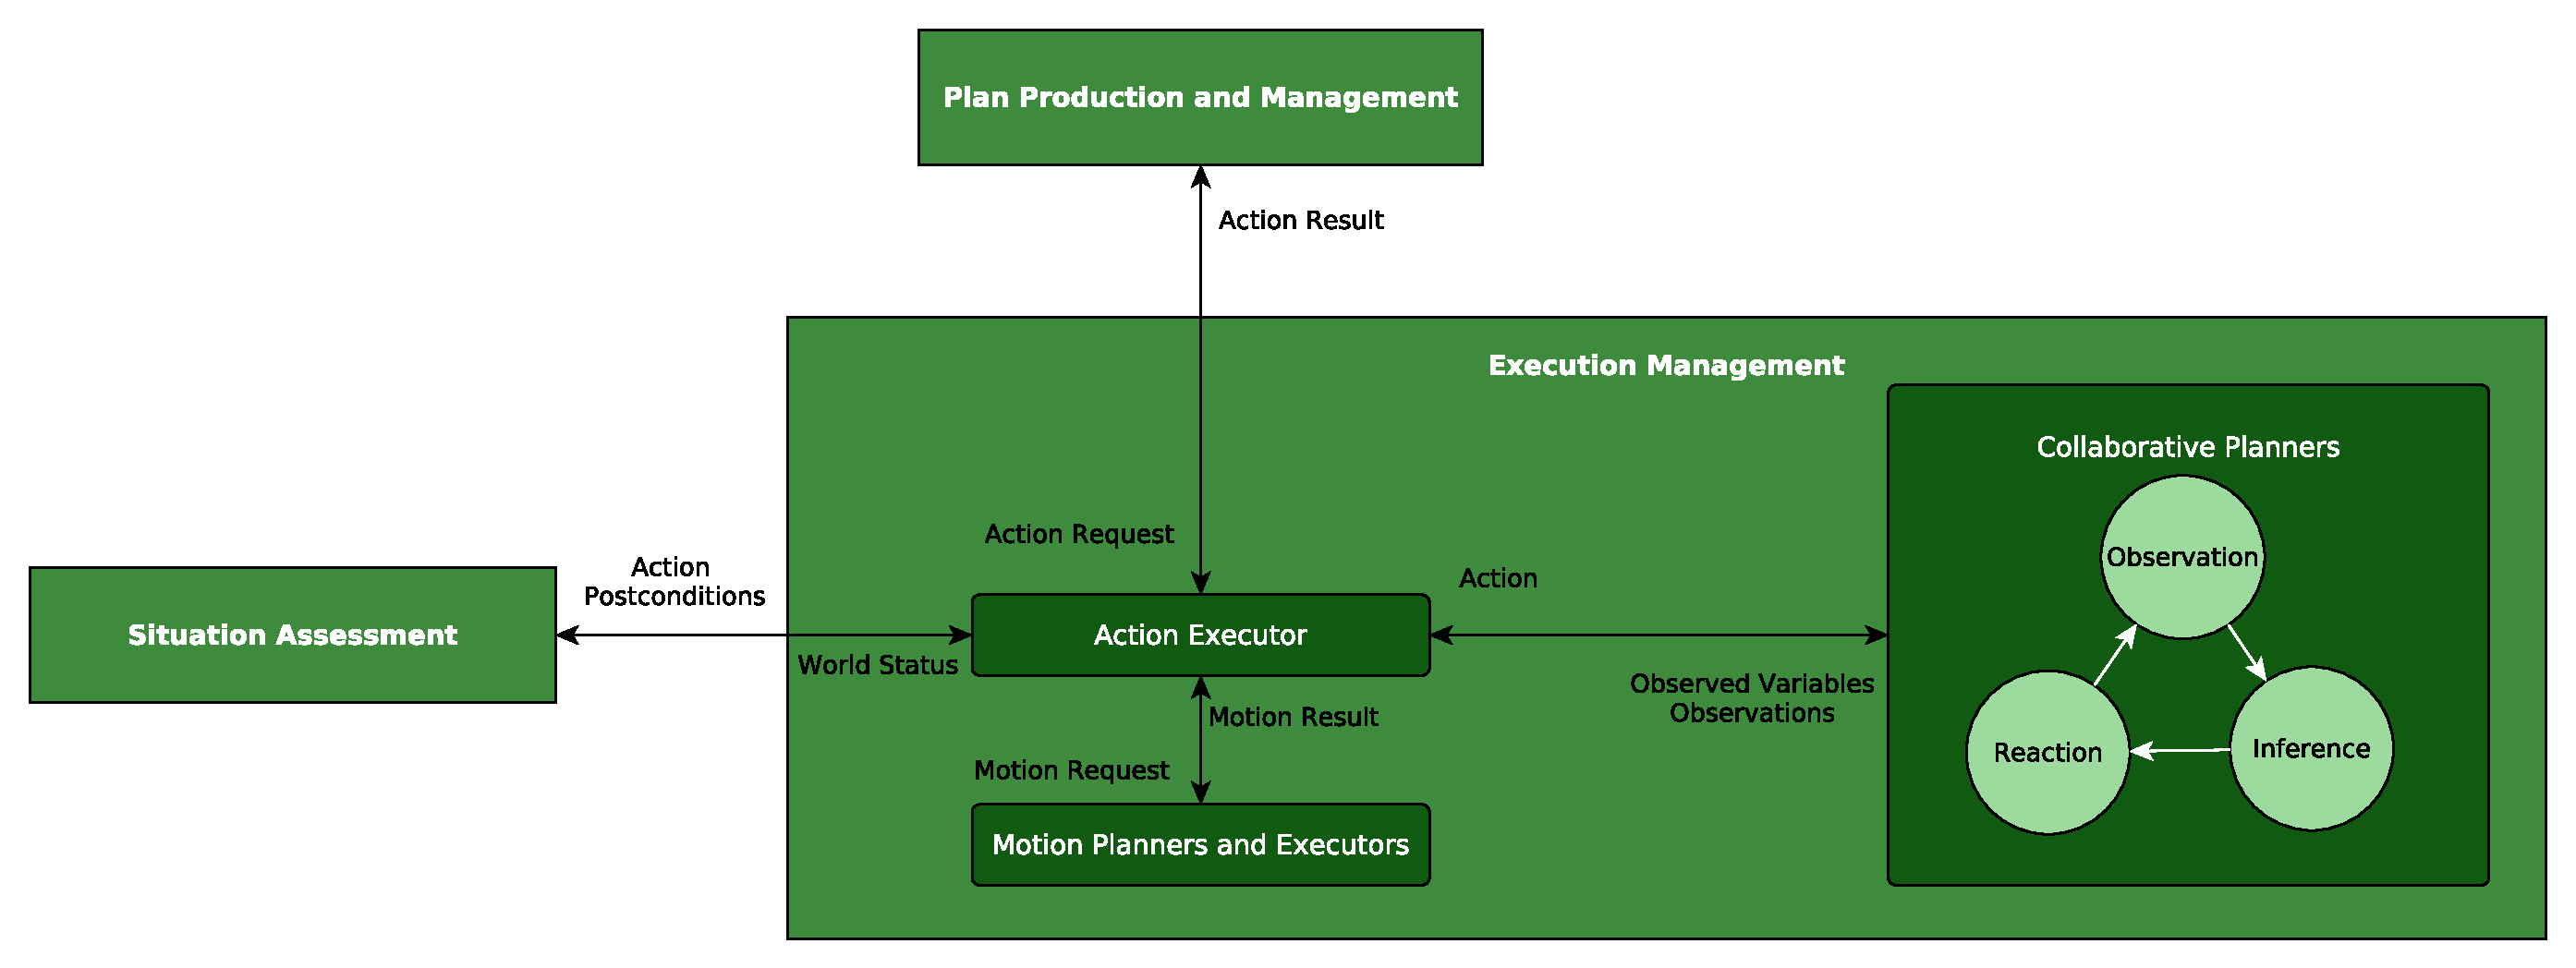
\includegraphics[clip,scale=0.38]{img/plan_execution/architecture.pdf}
	\caption[The architecture of the Execution Management layer]{The architecture of the Execution Management layer. Dark green rectangles represent modules, while light green rectangles layers. Arrows represent message exchanged between components, with the label detailing the message. The white ellipses represens, and their arrows, represent the process of the Collaborative Planners, explained in Section \ref{sec:plan_execution-collaborative_planners} }
	\label{fig:plan_execution:architecture}
\end{figure}

%fix figure


Parts of this chapter where presented in~\cite{fioreiser2014}.

\section{Action Executor}
\label{sec:plan_execution-action_executor}
The action executor handles action requests from the Plan Production and Management layer. Each action, as explained in subsection~\ref{sec:situation_assessment-belief_management}, is a tuple $(name, preconditions, target, postconditions)$. The execution of an action is handled in several steps:
\begin{itemize}
\item Check Preconditions. The system can check if the preconditions of the actions are valid by sending a query to the Situation Assessment layer. If the preconditions are not valid, the module returns an error.
\item Execute Action. The action is executed, by communicating with the Motion Planners and Executors and, if the current action is a joint action, with the Collaborative Planners.
\item Set Postconditions. After the action is completed, its $postconditions$ are set in the Database of the Situation Assessment Layer.
\end{itemize}

The execution of an action can fail, and in that case the world status is updated consequently. For example, if the robot was trying to pick an object, and the action fails because the robot can not find a motion to grab it, the object will be considered as \textit{not reachable} by the robot in the current world status. When the Plan Management and Production replans, the system could look for a plan where the robot changes position and tries again the pick, or even asks another agent to give him the object.

Actions can be paused and resumed, for example because a human steps in the trajectory planned by the robot. The robot is also able to show some social clues during an action, for example by moving its head toward the action's $target$. 

\section{Collaborative Planners} 
\label{sec:plan_execution-collaborative_planners}
When executing joint actions with humans, the robot needs to continuously observe its partner and react appropriately. The robot's action should be based on different aspects. First of all, the robot should act differently depending on the current status and level of advancement of the task. Second, the robot should consider the status of the world, in order to take appropriate actions. Then, as we said, the robot should observe its partner's behavior, which can give different information. Of course, the robot should coordinate with the human's movements. For example, if the two agents are performing an handover, and the human extends his hand, the robot should extend its arm to bring the object in a reachable position.

Observing the human's action can give us more subtle information, that represent how much he is engaged in the task. For example, in the case of the handover, if the human is oriented toward the robot and extending his hand, we can assume that the human is currently engaged and cooperating. If, instead, the human is looking in another direction, or moving away, we can infer that he is currently doing something else, and perhaps has even abandoned the task.

To reason on all these variables and produce an appropriate reaction, we introduced a special framework to manage cooperative actions, called the Collaborative Planners, based on hierarchical Mixed Observability Markov Decision Processes (MOMDP). Using an MOMDP we can model both observed variables, like the task and world status, and hidden variables, like the engagement level of the human, which we can measure from observations. Using a hierarchy of models, as explained in \cite{pineau2001hierarchical}, we can represent complex scenarios and tasks with smaller, simpler models, that can be solved more easily, and expand them by adding more actions and complex behaviors as we see fit.

When the system is executing a joint action between the robot and a human, the Action Executor will contact the related Collaborative Planner.  The Action Executor will send requests containing the observations and observed variables, used to update the MMODPs, and the planner will return a sub-action to execute. To maintain this model generic the Collaborative Planners will output high-level actions, which the Action Executor will adapt to the current situation. This process will continue until the planner reaches a goal states, chooses to abandon the task, or there is a failure.

For example, if the robot is giving a bottle to a human, the related Collaborative Planner will receive information such as the human's distance, orientation, and the pose of his arm, in order to compute if he is involved in the action. Depending on these information, the planner could choose high-level actions like \textit{continue}, which would prompt the robot to extend its arm or release the bottle, 

\subsection{Handover Collaboration Planner}
\label{subsec:case_study-helper-handover}
We implemented a MOMDP model to handle handovers between humans and robots. This model will output high-level actions, adapted by the Action Executor, depending on the current situation. Decisions will be made based on the following variables:

\begin{itemize}
\item The status of advancement of the task. This variables, whose values are \textit{\{not\_completed, touching, completed\}}, is set by the Action Executor module, in the Execution Management layer, depending on the current advancement of the task. The variable will be set as $completed$ when the handover has been performed, $touching$ when the robot detects pressure on the gripper used for the handover, and $not\_completed$ otherwise. 
\item The quality of commitment of the user. This variable has the same meaning as in the collaborative planner for guiding presented in \ref{subsec:case_study-spencer-collaborative_guide_planner} and can assume the same values, but is estimated from different variables. We will still consider the distance and orientation of the human toward the robot, but also the pose of its arm, particularly if its extended toward the robot. 
\item A timer. The variable is used in the same way as in the collaborative planner for guiding, presented in subsection~\ref{subsec:case_study-spencer-collaborative_guide_planner}.
\end{itemize}

The possible actions of this model are the following:
\begin{itemize}
\item Continue. The Action Executor will continue with the handover, which, depending on the situation, will prompt the system to extend the arm or activate the gripper.
\item Wait. The system will wait for the user if he is not engaged in the task.
\item Abandon. The system will abandon the task when the user is no longer interested in performing it. 
\end{itemize} 

 
\chapter{Human-Aware Probabilistic Planning}
\label{subsec:plan_management-happ}

\lhead{Chapter 7. \emph{Human-Aware Probabilistic Planning}} % Change X to a consecutive number; this is for the header on each page - perhaps a shortened title


\section{Introduction}
In some situations, the environment, or other agents' actions, can be very unpredictable, and the system needs to constantly adapt its plans to the current state of the world, by replanning or repairing processes, which can be expensive. To deal with this issue we developed a Human-Aware Probabilistic Planner, based on MDPs. Our goal is replicating the characteristics of HATP in a probabilistic domain. We designed this planner with the following ideas:

\begin{itemize}
\item Centralization. We will use a single planner, which chooses actions for all the involved agents.
\item Hierarchical. The domain will be split in different modules, which interact to solve the issue. Hierarchical models allow us to speed up the computation of the MDP policy, to reuse models in different domains and tasks, and can be helpful to produce HTN-like tree structures, which can be used in plan explanation and monitoring.
\item Tightly Coupled. We will focus on problems where the agents' interactions are frequent.
\item No Communication. The planner will  assume that all the agents have perfect knowledge of the world state. The rest of the system will have to take care of maintaining users' knowledge, ensuring the correct execution of the plan. Current planners that try to include communication issues often focus on loosely coupled interactions between the agents, in order to simplify the domain and be able to compute a policy for the problem. Since we choose to focus on tightly coupled problems, we can not use this solution, and so prefer to avoid the issue at this level.
\end{itemize}


\section{Single-Agent MDP}
The starting point for this planner is the single agent MDP. We start with the classical model $(S,A,T,C,G,S_0)$, where $S$ is the system space, $A$ is the set of actions, $T(s_i,a,s_j)$ is the probability to transition from state $s_i$ to state $s_j$ after taking action $a$, $C(s,a)$ is the cost of taking action $a$ in state $s$, $G \in S$ is the set of goal states, and $S_0 \in S$ is the set of starting states. We express the state space $S$ of the system as a set of variables $var$, each one with a possible range of values $values(v)$, where $v$ is a variable.

 We develop this model in the following way.

\subsection{Parameters}
We can define parameters in our MDP, and assign them to different values. We will call the list of parameters of an MDP $par$ and their current instantiation the \textit{parameter\_instance} of the model. Parameters can be linked to variables and values. We call $par\_var$ the variables associated to a parameter. 

For example, let's imagine a scenario of a room, with different furnitures and object. Let's define the state space of a generic MDP to take an object in this room. We can consider as variables the location of the agent, \textit{agent\_isAt}, which can assume value in the set ${f_1, f_2, f_3}$, where $f_i$ represent a furniture in the room. We can define an object variable, \textit{object\_isAt}, which can assume the same values as the \textit{agent\_isAt} variable. If we define two parameter variables, \textit{agent} and \textit{object}, and link them to the \textit{agent\_isAt} and \textit{object\_isAt} variables, we can create a generic MDP which can be used to plan for any agent (with similar capacities) to take an object in this room.

The MDP receives as input, when consulted to select an action, the state of the world,  which we will call \textit{real\_space}. The \textit{real\_space} will be converted, using the \textit{parameter\_instance}, to the \textit{parameter\_space}, which will be actually used by the model in its computations. 

For example, in the real world, we have two agents, \textit{Bob} and \textit{Greg}, and three objects \textit{glue}, \textit{book}, \textit{smartphone}. If we assign the \textit{agent} parameter to \textit{Bob} and the \textit{object} parameter to \textit{book}, when receiving the complete world state the MDP will assign as \textit{agent\_isAt} the location of Bob, and as \textit{object\_isAt} the location of the book, discarding unneeded variables.

Parameters allow us to create smaller, generic MDPs, which can be reused easily.


\subsection{Actions and Macro Actions}
We define actions as a tuple $(subject,action\_name,object,target)$, where each element of the tuple is called an $action\_part$.  We represent the action as a string, composed by its $action\_parts$, joined by the character `\_' as delimiter. We define the function $convertPar(a)$ and $convertReal(a)$ to convert action $a$ to the \textit{real\_space} or the \textit{parametrized\_space}.

We add to the normal set of actions of an MDP \textit{macro actions}, linked to other MDPs, which allow us to create a hierarchy of MDPs. We call $M$ the set of \textit{macro actions} of the MDP, and $sub(a)$ the sub-MDP linked to the \textit{macro action} $a$.

\section{Name and Parameter Name}
We define for each MDP class a \textit{name}, which identifies it, and a \textit{parametrized\_name}, which substitutes parameters using the \textit{parameter\_instance}. The \textit{name} is defined using the same tuple as an action. 

For example, an MDP whose goal is to obtain an object could have as \textit{name} $agent\_get\_object$ and as \textit{parametrized\_name}, in a certain moment, $Greg\_get\_book$.

We define a function $assignParameterFromActionName(a)$ which creates the \textit{parameter\_instance} of the MDP based on an action name. This function can be very useful when using \textit{macro actions}, by assigning parameters to the MDP from the \textit{macro action} and then consulting the sub-MDP.

For example, if the \textit{macro action} $Greg\_get\_book$ is linked to the $agent\_get\_object$ MDP, this function would assign to the $agent$ parameter the value $Greg$ 
and to the $object$ parameter the value $book$.

Each \textit{name} can be divided in a number of $name\_parts$,  with the same procedure as actions. The \textit{parametrized\_name} is divided as well in $parametrized\_parts$.


\subsection{Abstract States}

In some situations, a model might not need to base its planning choices on all the possible range values of a variable in the \textit{real\_space}. Imagine, for example, the case where an agent needs to perform a series of operations on the furniture $f_1$ in the room. In this case, we could model the  values of the \textit{agent\_isAt} variable as ${f_1 , other\_location}$, greatly reducing the state space. In this situation we say that \textit{agent\_isAt} is an \textit{abstract variable}. 

We build a map $abstract\_values_v$ for each abstract variable $v$, which links real world values to model values (e.g. $f_2 \rightarrow other\_location$). This map will be used to convert a state expressed in the $real\_space$ to the $parameter\_space$ of the model. 
%The choice of using abstract variables needs to be carefully weighted, because they can impact on the quality of the solution of the model.

\section{Multi-Agent MDP}
Now we will explain how we build a Multi-Agent MDP (MAMDP), starting from $n$ single-agent models, one for each agent. We will call the single-agent models $MDP_i$, where $1 \leq i \leq n $ is the index of the agent. In the following paragraphs, we will use the notion $S_i, var_i, values_i, A_i, T_i, C_i, G_i, S_{0i}, M_i, par_i, par\_var_i$ when referring to components of the single-agent MDP, adding the $i$ index to differentiate them from the MAMDP. 
 
\subsection{Name and Parameter Name}
The \textit{name} and \textit{parameter\_name} of the MAMDP are built by concatenating those of its agent MDPs, adding the `-' character to separate the single agents.

For example, the \textit{name} of MAMDP with single-agent models \textit{agent\_get\_object} and  \textit{agent\_clean\_table} is \textit{agent\_get\_object-agent\_clean\_table}.

\subsection{State Space and Parameters}
$par=\bigcup_{1 \leq i \leq n, p \in par_i} p+\text{`p'}+i $. \\
$par\_var=\bigcup_{1 \leq i \leq n, v \in par\_var_i} \> rename(v)$ \\
$var=\bigcup_{i=1}^{n}(var_i \setminus par\_var_i) \cup par\_var$ \\
$\forall_{v \in var}\> value(v)=\bigcup_{i| v \in var_i} 
\begin{cases}
	 value_i(v) \quad \text{if } v \not \in par_i \\
	 p+\text{`p'}+i \quad \text{if } v \in par_i \\
\end{cases}$ \\ 

To create the set of parameters of the MAMDP we will rename each parameter in the single-agent MDPs, adding an identifier composed by `p' and by the index of the MDP. We make this choice because different MDPs could share the same parameters, but they could be assigned to different values, and so need to be treated as separate entities, even if they have the same semantic meaning. Parameter variables are created by renaming the parameter variables of the sub-MDPs to account for this newly added identifier.

For example, if the $MDP_1$ model has a parameter \textit{object}, linked to a variable called \textit{object\_isAt}, we will rename the parameter as \textit{objectp1} and the variable as \textit{objectp1\_isAt}. 

We defined $S$ as the union of the variables of the single-agent MDPs excluding their parameter variables. We will instead take the parameter variables of the MAMDP, in the way that we just defined.

The MAMDP variable can assume all the possible values that are available in the corresponding variables of the sub-MDPs. As before, we will change values that are parameters to account for our renaming procedure. 

We define the function $single_i(s)$ , which converts the MAMDP state to state of the single-agent MDP $i$.


\subsection{Actions}
$A=(\prod_{i=1}^{n} A_i) \cup JointActions \cup WaitActions$ , where $JointActions$ is the set of collaborative actions, and $WaitActions$ is a set computed by enumerating all the possibile instances where one or more agents do not act, and simply wait, while others are acting.

The actions of the MAMDP are a concatenation of the actions of the single MDPS, adding the separator character `-' between the different agents actions. We will refer to the single agent actions of action $a$ as $a_i \quad \forall \> 1\leq i \leq n$.

For example, the MAMDP will contain actions such as `agentp1\_move\_surface1-agentp2\_move\_surface2'.

We add to $A$ the special set of $JointActions$, which are actions that the agents can use to cooperate. For example, if there is a resource in a single agent MDP which two agents can possess, we introduce a $handover$ action between them. 

For each $a \in A$, if there is a sub-action $a_i$ which is a macro action for MDP $i$, we create a new MAMDP and assign it as sub-MAMDP of $a$. This sub-MAMDP will be created from $n$ MDP models, as for its father, in the following way. Let $f$ be the father MAMDP, $c$ the sub-MAMDP, and $a$ the macro-action of $f$. \\
 $ \forall_{\text{MDP}\> m_i \in f}$ we assign an MDP $m_j$ in $c$ where:\\
$m_j= \begin{cases}
	m_i & \quad \text{if } a_i \not\in M_i \\
	sub_i(a_i) & \quad \text{if } a_i \in M_i 
\end{cases}$ \\

\subsection{Transition Function}
$T(s_a,a,s_b)=
\begin{cases}
\prod_{i=1}^{n}(T_i(single_i(s_a),a_i,single_i(s_b))) & \> \text{if } !isIncongruent(s_a) \land  !isIncongruent(s_b)  \\
0   & \quad \text{else}
	\end{cases}$ \\

The transition function is computed as the product of the transition functions of the single agent MDPs, on the converted states and actions.

We set the probability as zero if either the starting or ending states state of the transition are incongruent. This is done by converting the states to the \textit{real\_space} and checking the values of the different variables. We say that a state is incongruent if two non abstract variables in the \textit{parameter\_space}, that are assigned to the same \textit{real\_space} variable, have different values. If one or both the variables are abstract we check if their $abstract\_values$, for the current variable values, have a value in common. If not, we consider the state incongruent.

For example, consider the state $(objectp0\_isAt=`surface', objectp1\_isAt=`table', agentp0\_isAt=`table', agentp1\_isAt=`table')$. If in the current \textit{parameter\_instance} both \textit{objectp0} and \textit{objectp1} are assigned to the same variable, this state will be incongruent.

Consider now the state $(objectp0\_isAt=`agentp0', objectp1\_isAt=`other', agentp0\_isAt=`table', \\ agentp1\_isAt=`table')$. If $agentp0$ is a parameter assigned to $Greg$, and \textit{objectp1\_isAt} is an abstract variable whose \textit{abstract\_values} include $agent1$, this state will not be considered incongruent.  

\subsection{Cost Function}
$C(s_a,a,s_b)= 
	\begin{cases}
		max_{i=1}^{n}(C_i(single_i(s_a),a_i,single_i(s_b))  & \quad \text{if } s_b \not\in G \\
		\sum_{i | single_i(s_a) \in G_i} expectedCost_i(single_i(s_a))  & \quad \text{if } s_b \in  G
		\\
	\end{cases} $	\\

where $expectedCost_i(s)$ is a function that computes the expected cost for agent $i$ to reach a goal state by starting in state $s$ and following the action policy. In this calculation, we allow from the other agent only $JointActions$ that are necessary to solve the plan (e.g. handovers if the agent does not have a needed resource).

The cost function of the MAMDP is chosen by taking the maximum cost of the single agent actions that are executed, if the state $s_b$ is not a goal state. If it is a goal state, we take as cost an estimation of the time required by the other agents to complete their tasks, with only minimal cooperation. In this way, we encourage the MAMDP to choose plan where the agents cooperate and do not only try to achieve their goal.

\subsection{Start and Goal States}
$S_0=\bigcap_{i=1}^n S_{0i}$. The starting states of the MAMDP is set to the intersection of the single agents starting states.\\\\$G=\bigcup_{i=1}^n G_i $, where $G_i$ is the set of goal states of a single agent MDP. The goal states of the MAMDP is the intersection of the single agent goal states. The idea of this choice is that an MAMDP terminates when one of the agents has achieved its goal. 

\section{Example}
In this section we will show an example of creation of a MAMDP. We start by presenting a cooperative scenario. The robot and a human are working together to assemble three brackets on three differents work surfaces. To assemble a bracket the agents need to clean the surface, apply some glue to it, and fix the bracket. A possible set-up for this scenario is shown in figure ~\ref{fig:plan_management-mamdp_scenario}.

 \begin{figure}[ht!]
	% \centering
	\includegraphics[scale=0.5]{img/plan_management/mamdp_scenario.pdf}
	\caption[MAMDP example scenario]{The image shows the set-up for this example scenario. The four locations are represented as different rectangles and the objects as circles. }
	\label{fig:plan_management-mamdp_scenario}
\end{figure}

We start by defining a single-agent MDP for this scenario. We will use a hierarchical architecture, as shown in figure ~\ref{fig:plan_management-mamdp_single_mdp_architecture}. This architecture is composed by three different modules: AssembleAllBrackets, which controls the flow of the scenario; AssembleBracketSurface, which assembles a chosen bracket on a chosen surface; and GetObject, which obtains an object. We will create some simplifications in these models, as they are chosen just to explain how we build a MAMDP, and not for a realistic use.

\begin{figure}[ht!]
	% \centering
	\includegraphics[scale=0.5]{img/plan_management/mamdp_single_mdp_architecture.pdf}
	\caption[MAMDP example single MDP]{The image shows the architecture for the single agent MDP of the MAMDP example scenario. The various MDPs are represented as rectangles. The arrows show the links between hierarchical modules in the architecture. The label of the arrow shows the macro action corresponding to the link}
	\label{fig:plan_management-mamdp_single_mdp_architecture}
\end{figure}


\subsection{AssembleAllBrackets} 
\begin{itemize}
	\item $name: agent\_assembleallbrackets$.
	\item		$par: agent$
		\begin{itemize}
			\item $par_var(agent)=agent\_isAt$
		\end{itemize}
		In this example, we decided to create generic models which can plan either for greg or for the robot.
	\item $S:\;\{agent\_isAt,bracket1_isAt,bracket2_isAt,bracket3_isAt,surface1\_status,surface2\_status,surface3\_status\}$. 
		\begin{itemize}
			\item $values(agent\_isAt):\{table,surface1,surface2,surface3\}$.
			\item $values(bracketi\_isAt):\{table,surface1,surface2,surface3,agent,other\_agent\} \forall_{i=1}^3$. 
			\item $values(surfacei\_status):\{completed,other\_status\}\;\forall_{i=1}^3$.
		\end{itemize}
		\begin{itemize}
			\item $abstract\_values\_surfacei\_status:$ 
				\begin{itemize}
					\item $none: other\_status$.
					\item $cleaned: other\_status$.
					\item $glued: other\_status$.
				\end{itemize}
			\item $abstract\_values\_bracketi\_isAt$ 
				\begin{itemize}
					\item $greg: other\_agent$.
					\item $robot: other\_agent$.
				\end{itemize}	
		\end{itemize}
		The state set of the model contains the location of the agent, of the brackets, and the status of the surfaces. The agent and the objects can be located at the table or at one of the surfaces. In addition, objects can be possessed by another agent. The status of a surface can be set to none, meaning that the fixing process as not started; cleaned, meaning that the agent has already cleaned the surface; glued, meaning that the agent has applied glue to the surface; and completed, meaning the a bracket ha been fixed on it. 

		To simplify the model we consider the states $none,cleaned,glued$ as abstract states. We also consider $other\_agent$ as an abstract value, assigned to both agents present in the scenario. Let's consider, for example, that the instance of the \textit{agent} parameter is \textit{greg}, and that in the \textit{real\_space} \textit{bracket1\_isAt=greg}. It could seem that, when converting from converting from \textit{real\_space} to \textit{parameter\_space} the system would assign \textit{bracket1\_isAt} to \textit{other\_agent}, since \textit{other\_agent} is an abstract value for \textit{greg}. In reality, the system will give priority to the current parameter, and execute the conversion properly, by setting \textit{bracket1\_isAt=agent}. 
	\item $A:\;\{agent\_assemble\_bracketi\_surfacej\}\;\forall_{i=1}^1 \forall_{j=1}^3$.
	\item $M: A$.

	All of this model's actions are actually \textit{macros}.
	\item $G:\; \cup_{s:S} | \forall_{i=1}^3 surfacei\_status=completed\;\text{AND}\;forall_{i=1}^3\exists_{j}|bracketi\_isAt=surfacej \text{AND} \forall_{i=1}^3 bracketi\_isAt!=bracketj\_isAt.$

	The goal of this model is to fix all the brackets on the surfaces. To check this, we set as goal states every state in which the brackets are located on different surfaces and the status of each surface is \textit{completed}. 
	\item $S_0:\; \cup_{s:S} \exists{1\leq i \leq 3} | surfacei\_status!=completed$.

\end{itemize}

Note that we did not need to specify a cost function for this model. Since all of its actions are \textit{macros}, the cost function will be directly derived by its sub-models.

\subsubsection{AssembleBracket}
\begin{itemize}
	\item $name: agent\_assemble\_bracket\_surface$.
	\item		$par: \{agent,bracket,surface}$
		\begin{itemize}
			\item $par_var(agent)=agent\_isAt$
			\item $par_var(bracket)=bracket\_isAt$
			\item $par_var(surface)=surface\_status$
		\end{itemize}

	\item $S:\;\{agent\_isAt,bracket\_isAt,surface\_status,glue\_isAt}$. 
		\begin{itemize}
			\item $values(agent\_isAt):\{surface,other\_location}$.
			\item $values(bracket\_isAt):\{agent,surface, other\_location,other\_agent}$. 
			\item $values(glue\_isAt):\{agent,other\_location,other\_agent}$. 
			\item $values(surface\_status):\{none,cleaned,glued,completed}$.
		\end{itemize}
		\begin{itemize}
			\item $abstract\_values\_bracket\_isAt$ 
				\begin{itemize}
					\item $surfacei=other\_location \forall_{i=1}^n$ .
					\item $table=other\_location$.
					\item $greg=other\_agent$.
					\item $robot=other\_agent$.
				\end{itemize}	
			\item $abstract\_values\_glue\_isAt=abstract\_value\_bracket\_isAt$ 
			\item $abstract\_values\_agent\_isAt$
				\begin{itemize}
					\item $surfacei=other\_location \forall_{i=1}^n$ .
					\item $table=other\_location$.
				\end{itemize}
		\end{itemize}
		
		This state set will contain, other than the variables of \textit{AssembleAllBrackets}, also the location of the glue bottle. In this situation, \textit{surface_status} will not be an abstract variable, since the model needs to know what is the exact state of the fixing process. We greatly simplified the number of locations where agents and objects can be by using abstract variables. This model is only interested in knowing if the agent has an object (glue or bracket) or not. In the case where the agent does not have an object, it can invoke the \textit{get\_object macro}, which will take charge of obtaining it, using a more complete state space.
	\item $A:\;\{agent\_move\_surface,agent\_clean\_surface,agent\_glue\_surface,agent\_fix\_bracket,agent\_get\_bracket,agent\_get\_glue}$.
	\item $M:\;{agent\_get\_bracket,agent\_get\_glue}$.
	\item $G:\; \cup_{s:S} | surfacei\_status=completed$
	\item $S_0:\; \cup_{s:S} | surfacei\_status \neq completed$
\end{itemize}


\subsubsection{GetObject}
\begin{itemize}
	\item $name: agent\_get\_object$.
	\item		$par: \{agent,object}$
		\begin{itemize}
			\item $par_var(agent)=agent\_isAt$
			\item $par_var(object)=object\_isAt$
		\end{itemize}

	\item $S:\;\{agent\_isAt,object\_isAt}$. 
		\begin{itemize}
			\item $values(agent\_isAt):\{table,surface1,surface2,surface3}$.
			\item $values(object\_isAt):\{table,surface1,surface2,surface3,agent,other\_agent}$. 
		\end{itemize}
		\begin{itemize}
			\item $abstract\_values\object\_isAt$ 
				\begin{itemize}
					\item $greg=other\_agent$.
					\item $robot=other\_agent$.
				\end{itemize}	
		\end{itemize}
		
		This state set will contain, other than the variables of \textit{AssembleAllBrackets}, also the location of the glue bottle. In this situation, \textit{surface_status} will not be an abstract variable, since the model needs to know what is the exact state of the fixing process. We greatly simplified the number of locations where agents and objects can be by using abstract variables. This model is only interested in knowing if the agent has an object (glue or bracket) or not. In the case where the agent does not have an object, it can invoke the \textit{get\_object macro}, which will take charge of obtaining it, using a more complete state space.
	\item $A:\;\{agent\_move\_table, agent\_move\_surface1\, agent\_move\_surface2, agent\_move\_surface3, agent\_take\_object}$.
	\item $M:\;{\emptyset}$.
	\item $G:\; \cup_{s:S} | object\_isAt=agent$
	\item $S_0:\; \cup_{s:S} | object\_isAt \neq agent$
\end{itemize}

We will now show how our MAMDP is created. The MAMDP hierarchy, shown in figure ~\ref{mamdp_hierarchy} will contain different models. At the highest level lies the model \textit{AssembleAllBracket-AssembleAllBracket}, a duplication for two agents of the highest top module. The lowest modules include different combinations of the single agent sub-MDPs, in order to account for the possible task assignations. We will start by showing the top MAMDP model.

\subsubsection{AssembleAllBrackets-AssembleAllBrackets}
\begin{itemize}
	\item $name: agent\_assembleallbrackets-agent\_assembleallbrackets$.
	\item		$par: \{agentp1,agentp2\}$
		\begin{itemize}
			\item $par_var(agentp1)=agentp1\_isAt$
			\item $par_var(agentp2)=agentp2\_isAt$
		\end{itemize}

		The name of the parameters are changed, adding \textit{pi} at the end, where \textit{i} is the index of the agent. This allows to assign them in an unique way.
	\item $S:\;\{agentp1\_isAt,agentp2\_isAt, bracket1_isAt,bracket2_isAt,bracket3_isAt,surface1\_status,surface2\_status,surface3\_status\}$. 
		\begin{itemize}
			\item $values(agentp1\_isAt):\{table,surface1,surface2,surface3\}$.
			\item $values(agentp2\_isAt):\{table,surface1,surface2,surface3\}$.
			\item $values(bracketi\_isAt):\{table,surface1,surface2,surface3,agentp1,agentp2} \forall_{i=1}^3$. 
			\item $values(surfacei\_status):\{completed,other\_status\}\;\forall_{i=1}^3$.
		\end{itemize}
		\begin{itemize}
			\item $abstract\_values\_surfacei\_status:$ 
				\begin{itemize}
					\item $none: other\_status$.
					\item $cleaned: other\_status$.
					\item $glued: other\_status$.
				\end{itemize}
		\end{itemize}
		The state set is not very different, simply accounting for the presence of two agents.

	\item $A:\;\{agentp1\_assemble\_bracketi\_surfacej-agentp2\_assemble\_bracketk\_bracketl\}\;\forall_{i=1}^1 \forall_{j=1}^3
	\forall_{k=1}^3 \forall_{l=1}^3 \cup JointActions \cup WaitActions$.
	\item $JointActions=agentpi\_handover\_bracketj\_agentpl \forall_{i=1}^2 \forall{j=1}^3 \forall_{l=1; l!=i}^3$.
	\item $WaitActions=(agentp1\_assemble\_bracketi\_surfacej-agentp2\_wait \cup agentp1\_wait-agentp2\_assemble\_bracketi\_surfacej) \forall_{i=1}^3 \forall_{j=1}^3$.

	The action set is the cartesian product of the actions of the single models, plus two actions to exchange brackets, plus actions where only one agent is acting.
	\item $M: A$.
	\item $G:\; \cup_{s:S} | \forall_{i=1}^3 surfacei\_status=completed\;\text{AND}\;forall_{i=1}^3\exists_{j}|bracketi\_isAt=surfacej \text{AND} \forall_{i=1}^3 bracketi\_isAt!=bracketj\_isAt.$
	\item $S_0:\; \cup_{s:S} \exists{1\leq i \leq 3} | surfacei\_status!=completed$.

	The starting and goal states are the same as the single-agent model, since the two models used to create the MAMDP are the same the intersection and union of the states will be the same
\end{itemize}


If we would create and solve a new MAMDP for each of these macro, we would create a great quantity of models. Fortunately, as previously said, we can reduce this number by creating generic sub_models for a macro that can be used when there are not parameters in common. In this case, we actually need to create a single sub-MDP for every action of the type \textit{agentp1\_assemble\_bracketi\_surfacej-agentp2\_assemble\_bracketk\_surfacel}, where $i=j$ or $j=l$ (since they would have variables in common), plus a generic sub-MAMDP for all the other cases. Actually, in this case, these specific MDPs would not be created, since they are considered not valid, as the intersection of their goal states is null (since a bracket can not be on two surfaces at the same time and a surface can not contain more than one bracket).

Let us consider the AssembleBracket-GetObject MDP, deeper in the hierarchy. In this case, we will need to create a generic sub-MAMDP, plus specific MDPs for the macros \textit{agentp1\_assemble\_bracketi\_surfacej-agentp2\_get\_bracketi} and \textit{agentp1\_assemble\_bracketi\_surfacej-agentp2\_get\_glue}, since they share resources. We will show parts of this sub-MAMDP.  

\subsubsection{AssembleBracket-GetObject}
\begin{itemize}
	\item $name: agent\_assemblebracket-agent\_getobject$.
	\item		$par: \{agentp1,bracketp1,surfacep2,agentp2,objectp2\}$
		\begin{itemize}
			\item $par_var(agentp1)=agentp1\_isAt$
			\item $par_var(bracket1)=bracketp1\_isAt$
			\item $par_var(surfacep1)=surfacep1\_status$
			\item $par_var(agentp2)=agentp2\_isAt$
			\item $par_var(object2)=objectp2\_isAt$
		\end{itemize}

	\item $S:\;\{agentp1\_isAt, bracketp1\_isAt,surfacep1\_status, glue\_isAt, agentp2\_isAt, objectp2\_isAt}$. 
		\begin{itemize}
			\item $values(agentp1\_isAt):\{surfacep1,other\_location}$.
			\item $values(bracketp1\_isAt):\{agentp1,surface, other\_location,other\_agent}$. 
			\item $values(glue\_isAt):\{agentp1,other\_location,other\_agent}$. 
			\item $values(surfacep1\_status):\{none,cleaned,glued,completed}$.
			\item $values(agentp2\_isAt):\{table,surface1,surface2,surface3}$.
			\item $values(objectp2\_isAt):\{table,surface1,surface2,surface3,agentp2,other\_agent}$. 
		\end{itemize}
		\begin{itemize}
			\item $abstract\_values\objectp2\_isAt$ 
				\begin{itemize}
					\item $greg=other\_agent$.
					\item $robot=other\_agent$.
				\end{itemize}	
			\item $abstract\_values\_bracketp1\_isAt$ 
				\begin{itemize}
					\item $surfacei=other\_location \forall_{i=1}^n$ .
					\item $table=other\_location$.
					\item $greg=other\_agent$.
					\item $robot=other\_agent$.
				\end{itemize}	
			\item $abstract\_values\_glue\_isAt=abstract\_value\_bracketp1\_isAt$ 
			\item $abstract\_values\_agentp1\_isAt$
				\begin{itemize}
					\item $surfacei=other\_location \forall_{i=1}^n$ .
					\item $table=other\_location$.
				\end{itemize}
		\end{itemize}

	\item $G:\; \cup_{s:S} | surfacep1\_status=completed\; \text{OR} \; objectp2\_isAt=agentp2$
	\item $S_0:\; \cup_{s:S} | surfacep1\_status=completed; \text{AND} \; objectp2\_isAt \neq agentp2$

	The goal and starting states of the model are, respectively, the union and intersection of the single models.
\end{itemize}


Finally, to conclude, we show the special handover MAMDP, used for cooperative actions. Since this is a special model, not created by joining two single-agent MDPs, it will not follow the same rules, and instead it will be treated in a similar way as a single agent MDP.

\subsubsection{Handover}
\begin{itemize}
	\item $name: agent1\_handover\_object\_agent2-agent2\_receive\_object\_agent2$.
	\item		$par: \{agent1,object,agent2}$
		\begin{itemize}
			\item $par_var(agent1)=agent1\_isAt$
			\item $par_var(agent2)=agent2\_isAt$
			\item $par_var(object)=object\_isAt$
		\end{itemize}

	\item $S:\;\{agent1\_isAt, agent2\_isAt, object\_isAt}$. 
		\begin{itemize}
			\item $values(agent1\_isAt):\{surface1,surface2,surface3,table}$.
			\item $values(object\_isAt):\{agent1,agent2,other\_location}$. 
			\item $values(agent2\_isAt):\{surface1,surface2,surface3,table}$. 
		\end{itemize}
		\begin{itemize}
			\item $abstract\_values\object2\_isAt$ 
				\begin{itemize}
					\item $table=other\_location$.
					\item $surface1=other\_location$.
					\item $surface2=other\_location$.
					\item $surface3=other\_location$.
				\end{itemize}	
		\end{itemize}

	\item $A:\;\{agent1\_move\_location-agent2\_move\_location, agent1\_move\_location-agent2\_wait -agent1_wait-agent2\_move\_location, agent1\_give\_object\_agent2-agent2\_receive\_object\_agent1}\; \text{where}\; location \in \{table,surface1,surface2,surface3\}$
	\item $G:\; \cup_{s:S} | object\_isAt=agent2$
	\item $S_0:\; \cup_{s:S} | object\_isAt=agent1$
\end{itemize}


\subsection{Discussion}
The result of this fusion is an MDP, that can be solved with well-known algorithms, like value iteration. By fusing all the possible MDPs, the resulting model can be  very hard to solve but, using macro actions, parameters, and abstract states we can greatly reduce its complexity. 

The action space of the joint model is calculated as the cross product of the action spaces of the single model. When there are several macro actions in the agent models, this could result in the creation and computation of the policy of several sub-models, which can significantly slow down the computation of a solution for the model. We can reduce this process by making several considerations.

First of all, created MAMDPs can be reused in different branches of the hierarchy, if needed. When creating a new MAMDP, we will look to see if there is already an existing MAMDP with the same $name$ and, if so, we will use it.

Second, parameters can greatly  reduce the number of sub-MAMDPs to compute. Let $a$ be a \textit{macro action}, $c$ the sub-MAMDP linked to $a$, $1..n$ the indexs of the single-agent MDPs of $c$, which are selected as previously explained.

 We create the \textit{parametrized\_name} of $c$ by concatenating the \textit{parametrized\_name} of its single-agent MDPs. To set the $name$ of  $c$ we process each name of its single-agent MDPs $name_i$, by modifying all of its $name\_parts_{i,k}$, with $1 \leq k \leq m$ in the following way:\\
$name\_part_{i,k}=
\begin{cases}
	name\_part_{i,k} & \quad \text{if } !parametersInCommon(name\_part_{i,k}) \\
	parametrized\_part_{i,k} & \quad \text{else}
\end{cases}$ \\
where $parametersInCommon(name\_part_{i,k})$ is a function that returns true if $name\_part_{i,k}$ is a parameter in sub-MDP $i$, and there is a sub-MDP with index $j$, where $name\_part_{i,k}$ is a parameter or variable. \\

The idea behind this choice is the following. If the sub-MDPs do not have parameters in common, we can use a generic MAMDP to represent this instance. For example, if we create an MAMDP for the macro action $agent1\_clean\_table-agent2\_clean\_shelf$, we can use the MAMDP $agent\_clean\_furniture-agent\_clean\_furniture$ since the sub-MDP models do not have parameters in common, and their actions will not conflict.

 If instead we create an MAMDP for the macro action $agent1\_clean\_table-agent2\_clean\_table$ we create a specialized MAMDP, since there are parameters in common ($table$) and if we treat them as different objects there could be incongruences in the MAMDP planning. 
